\chapter{Поиск двойных и кратных звезд через анализ их изображений} \label{ch:ch4}
%улами~\ref{moments}
Представление изображения звезды в виде коэффициентов shaplete--разложения дает возможность на уровне математического формализма анализировать форму этих изображений, что открывает дополнительную возможность детектирования ранее неизвестных двойных и кратных систем. Такой анализ может с одной стороны применяться для верификации метода $\Delta\mu$-двойных, а с другой "--- перекрыть его некоторые <<слепые зоны>>. 
Стоит отметить, что идея анализа изображения звезд не нова и присутствует в современной научной литературе. К примеру, в работе \cite{2017MNRAS.468.3499D} представлены результаты поиска двойных звезд по оценке формы изображений. Основной критерий, рассматриваемый как фактор двойственности звезды, "--- это степень эллиптичности. Авторы отмечают, что метод работает для звездных систем с $\rho>0.3''$. На рисунке~\ref{fig:PanSt} представлен примеры результатов исследования в случае одиночной и двойной звезд.

\begin{figure}[h]
\centering
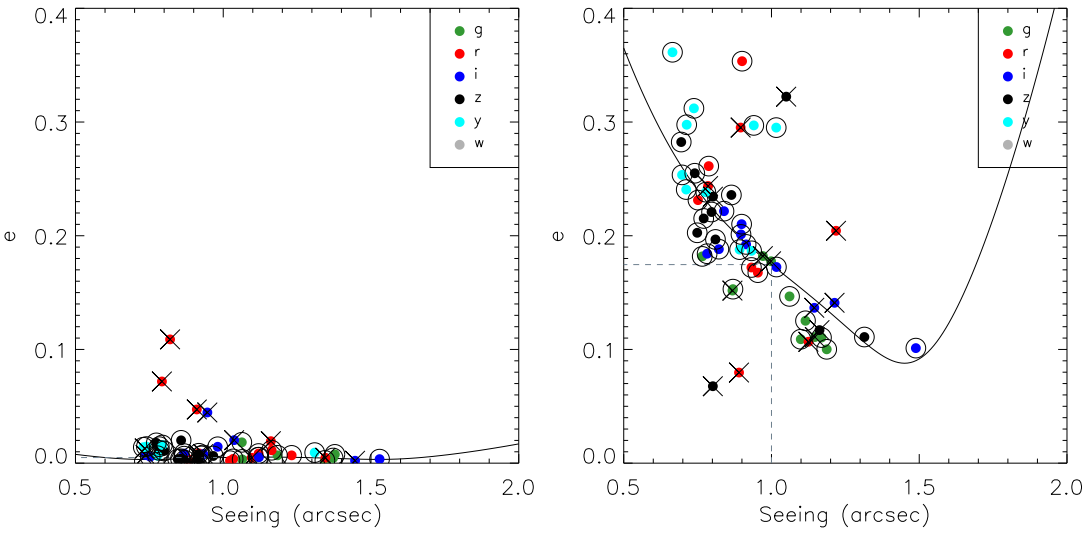
\includegraphics [scale=0.45] {Deacon-ellipticity}
\caption{Pan-STARRS – выявление двойных звезд по измерениям эллиптичности изображений \cite{2017MNRAS.468.3499D}. Слева – одиночная звезда, справа – двойная. Взято из \cite{2017MNRAS.468.3499D}, рис. 1.}
\label{fig:PanSt}
\end{figure}

Как уже упоминалось в главе~\ref{ch:ch2}, shapelet-разложение может служить мощным инструментом анализа форм изображений. 

Пользуясь формулами~(2.7)~--~(2.9), выразим эллиптичность и асимметрию изображения, которые могут служить маркерами двойственности.

Величины $q_{xx}$, $q_{yy}$, $q_{xy}$ из уравнений (2.7)~--~(2.9) позволяют определить эллиптичность изображения $e$ \cite{2017MNRAS.468.3499D}:
\begin{equation}
\label{eq:ell}
\left[e_1,~e_2\right] = \left[\frac{q_{xx}-q_{yy}}{q_{xx}+q_{yy}},~\frac{q_{xy}}{q_{xx}+q_{yy}}\right],\\
     e = \sqrt{e_1^2+e_2^2}.
\end{equation}

Один из возможных способов построения индекса асимметрии основан на повороте исходного изображения $I(x,y)$ на $180^\circ$. Таким образом получается развернутая копия исходного изображения $I(x,y)^{180}$. Далее индекс асимметрии вычисляется так \cite{2005MNRAS.363..197M}:
\begin{equation}
\label{eq:asy}
A = F^{-1}\cdot \sum_{pixels} |I(x,y)-I(x,y)^{180}|.
\end{equation}

В пространстве декартовых шейплет-коэффициентов поворот на $180^\circ$ осуществляется путем смены знаков для коэффициентов с нечетной суммой индексов $n_1+n_2$. Это наглядно показано на рис.~\ref{fig:rotate180}. В результате числитель в формуле для расчета индекса асимметрии можно определить из взвешенной суммы удвоенных коэффициентов $f_{n_1,n_2}$ с соответствующими индексами (то есть не прибегая к длительным вычислениям в пространстве изображений). 

Описанные во второй главе соотношения \ref{eq:shape-basis-functions} и \ref{eq:image-shapelet} демонстрируют, что информация о форме изображения содержится в коэффициентах $f_{n_1,n_2}$, которые не зависят от того, как центрировано изображение. Поэтому при вычислении индекса асимметрии с помощью шейплет-коэффициентов не требуется предварительно выполнять процедуру центрирования изображения. 

\begin{figure}[pt]
\centering
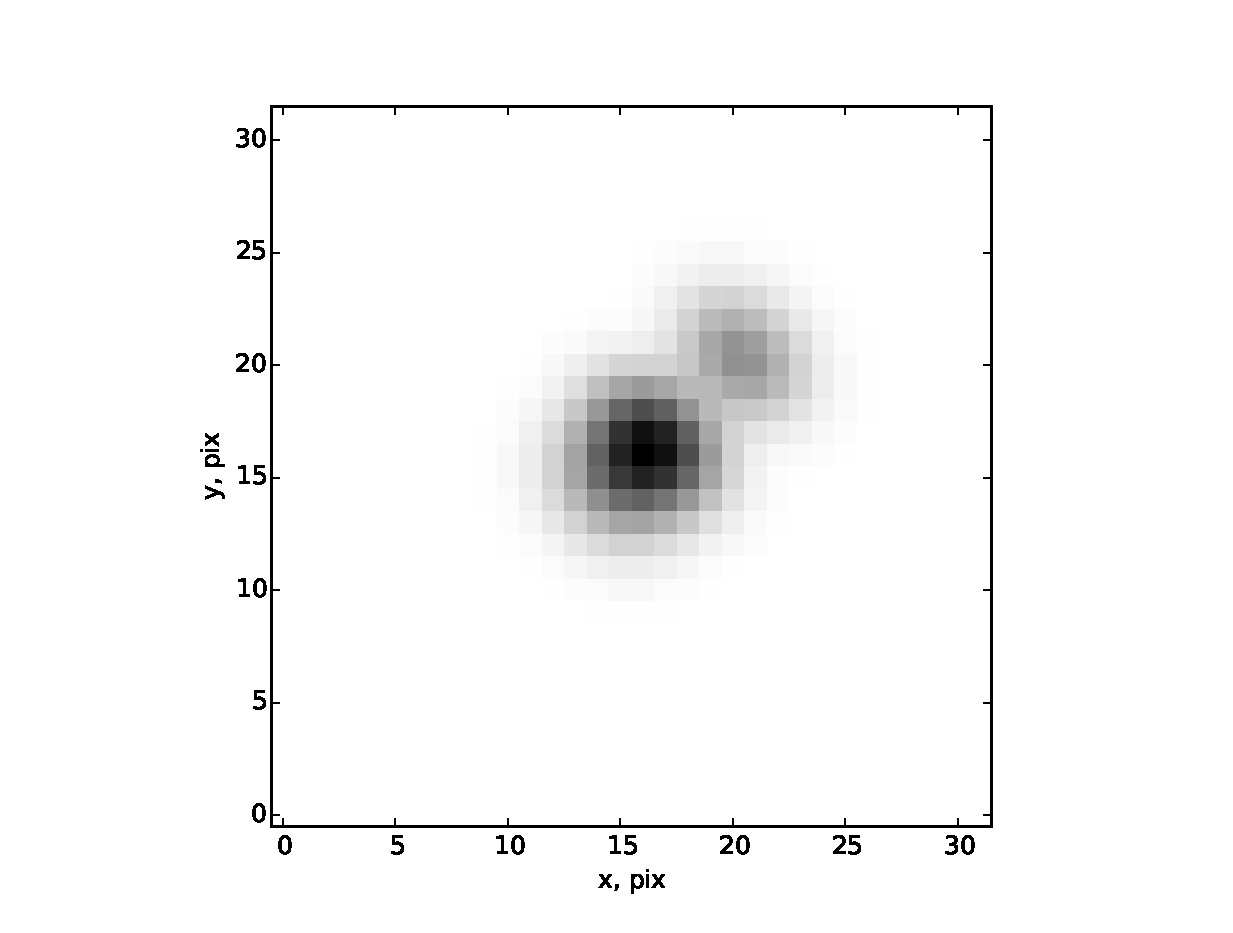
\includegraphics[width=0.458\textwidth]{asy-in.eps}
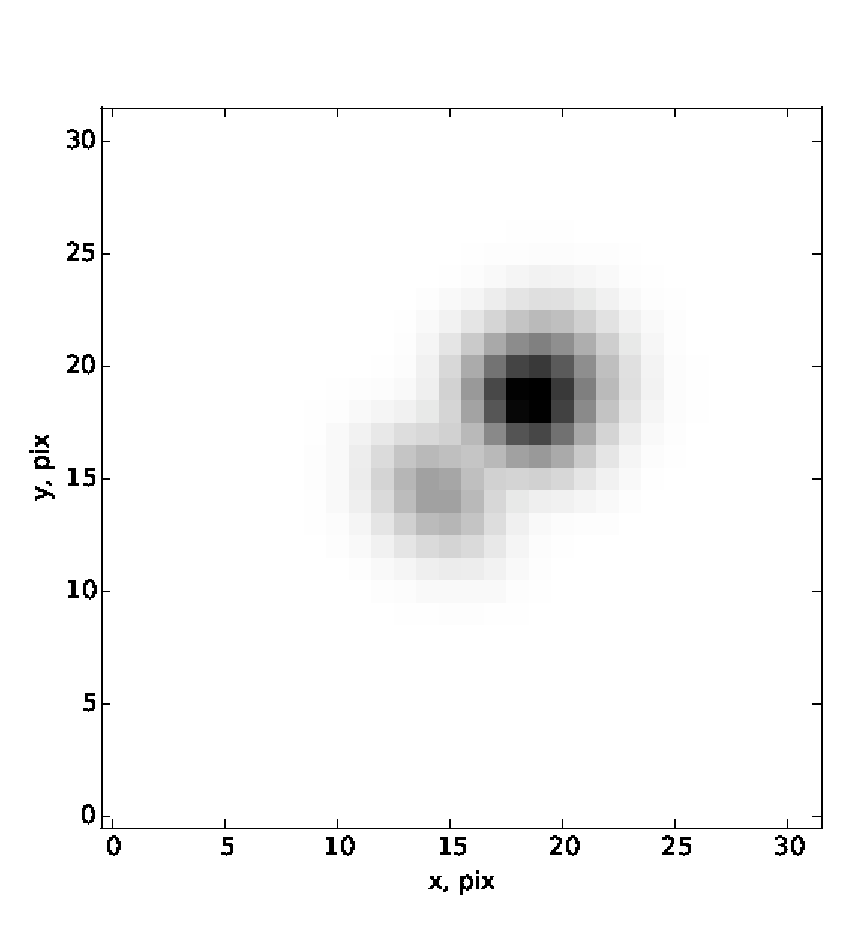
\includegraphics[width=0.458\textwidth]{asy-out.eps}
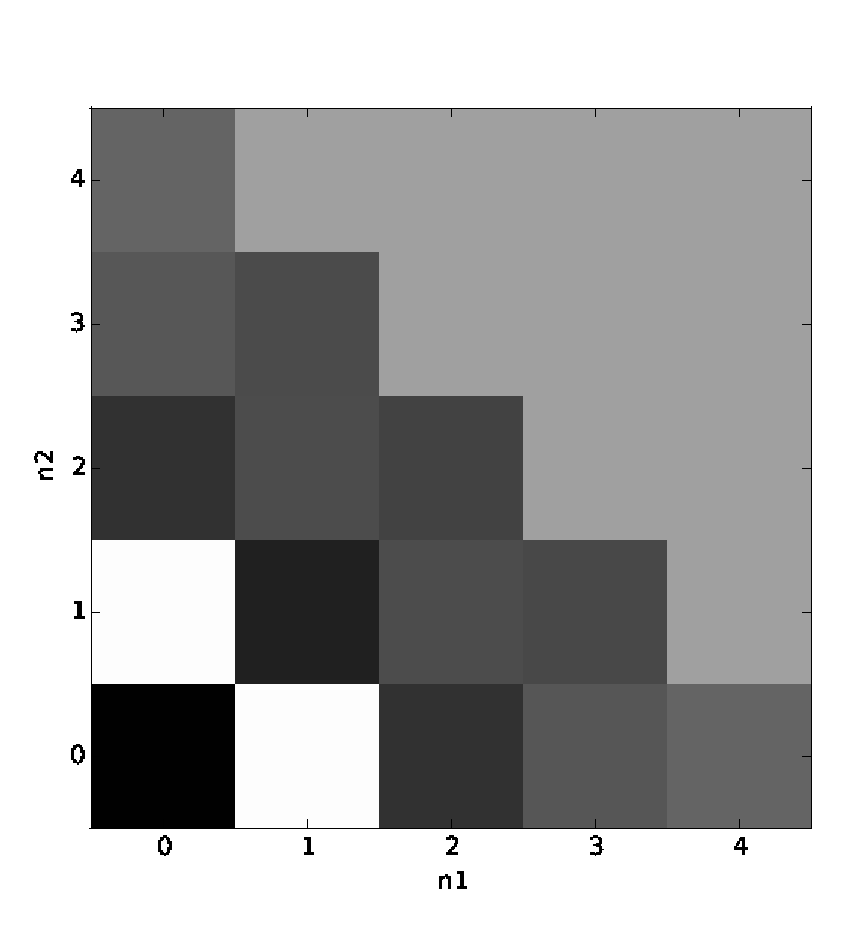
\includegraphics[width=0.45\textwidth]{portret-asy-in.eps}
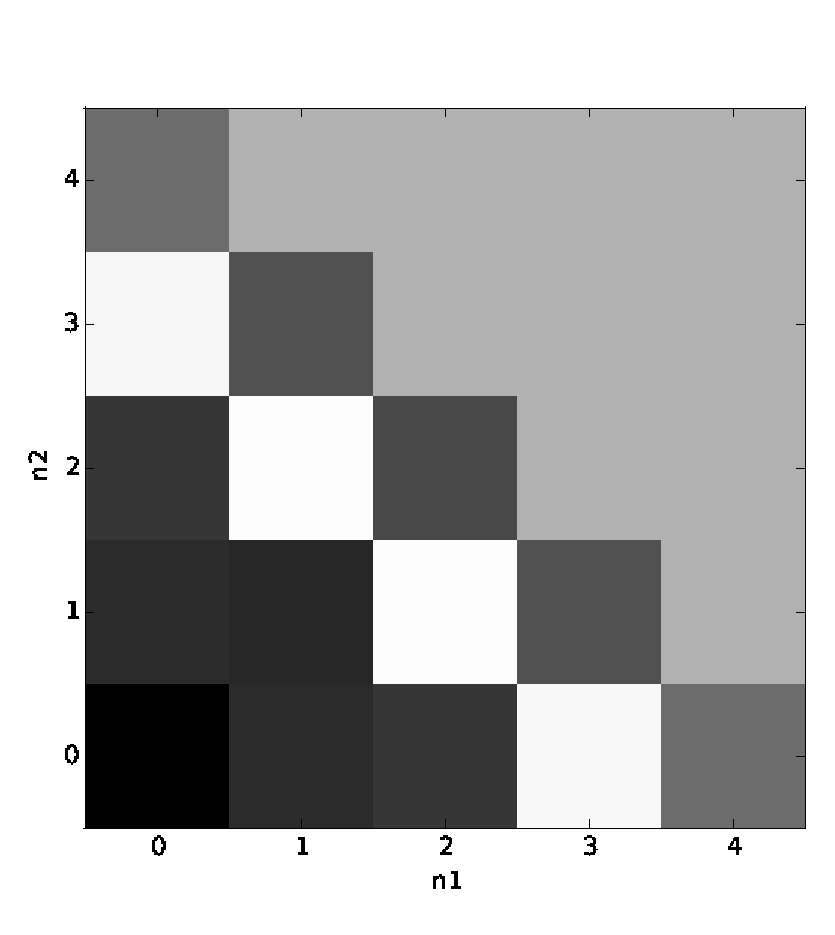
\includegraphics[width=0.45\textwidth]{portret-asy-out.eps}
%\setcaptionmargin{5mm}
%\captionstyle{normal}
\caption{Поворот изображения на $180^\circ$ путем смены знаков коэффициентов с нечетной $f_{n_1,n_2}$ суммой индексов (слева "--- исходное изображение, справа "--- результат поворота). Шейплет-коэффициенты, отвечающие прямому и развернутому изображениям, показаны под соответствующими рисунками. Взято из \cite{2018AstL...44..103K}, рис. 3.}
\label{fig:rotate180}
\end{figure}

Использование только оценок эллиптичности или только индекса асимметрии существенно снизит потенциал данной методики. Это хорошо видно из анализа данных на рис.~\ref{fig:bin-examples}. Если разность блеска компонент мала, то и индекс асимметрии будет близок к нулю. Зато значение эллиптичности будет значимым. И наоборот, при больших $\Delta m$ эллиптичность будет заметно падать, в то время как асимметрия будет расти.

\begin{figure}
\centering
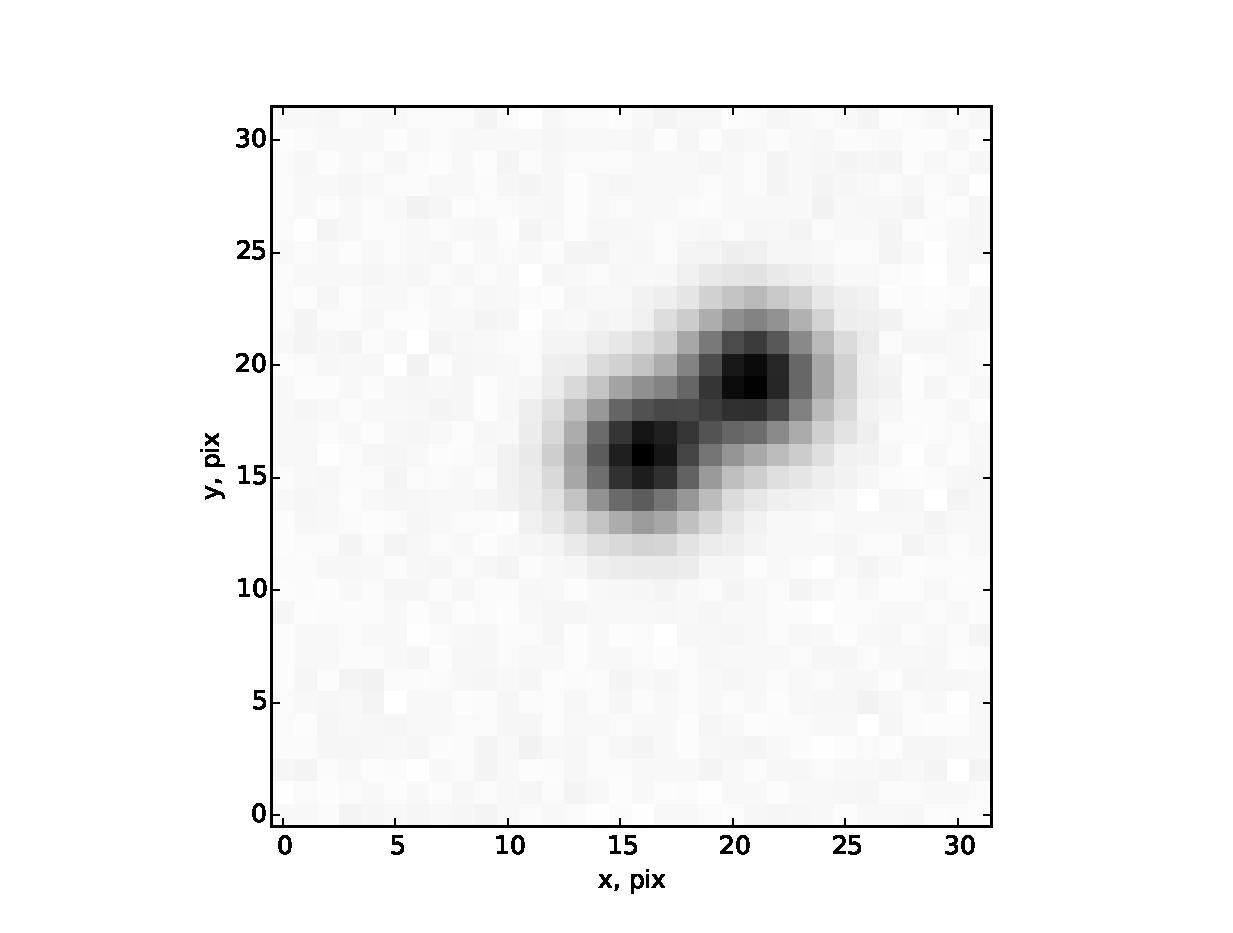
\includegraphics[width=0.48\textwidth]{asy_6_35_00_100_008_0410.eps}
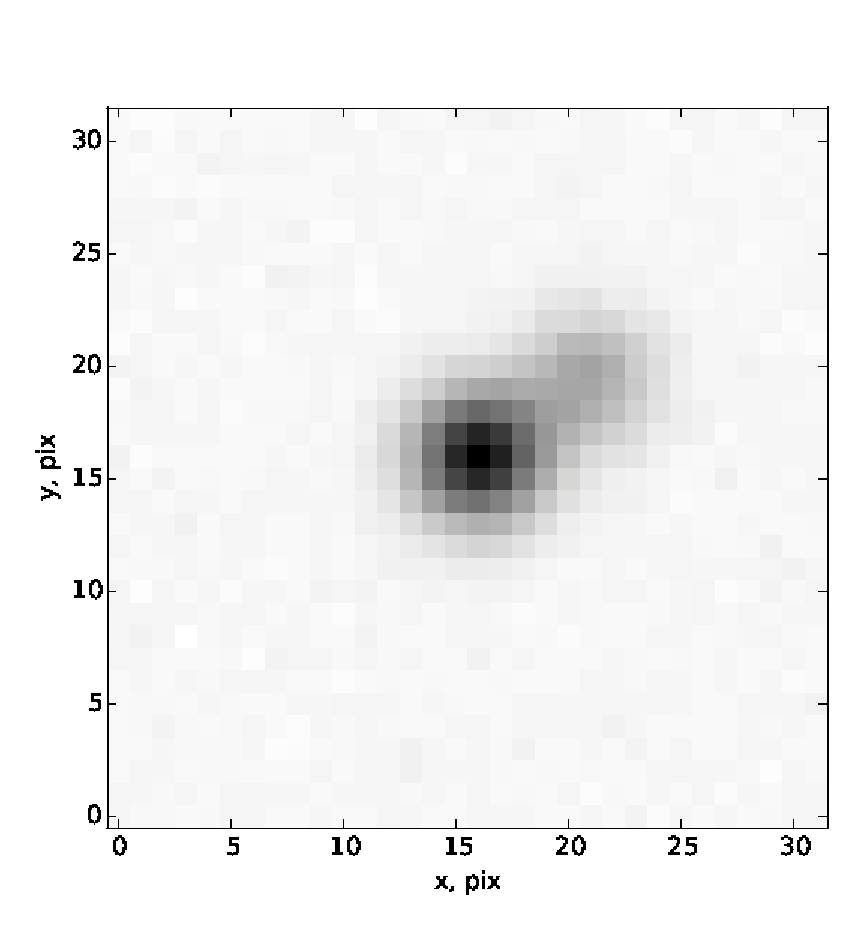
\includegraphics[width=0.48\textwidth]{asy_6_35_10_100_071_035.eps}
\caption{Модельные изображения двойных звезд. Слева система с параметрами $\rho=6~pix$, $\theta = 55^\circ$, $\Delta m=0^m$. Для нее $e_t = 0.41$, $A_t = 0.08$. Для системы справа при тех же пространственных параметрах, задано заметное различие блеска $\Delta m=1^m $. Для данной пары $e_t = 0.35$, $A_t = 0.71$. Взято из \cite{2018AstL...44..103K}, рис. 4.}
\label{fig:bin-examples}
\end{figure}

Методика анализа этих двух критериев кратности звезд применена и в Пулковской программе \cite{2018AstL...44..103K}. В качестве объектов исследования были выбраны 702 сравнительно слабые звезды с большими собственными движениями ($V>13^m$, $\mu>300''$/yr), для которых флаг <<duplicate source>> в каталоге Gaia DR1 равен единице. Распределение программных звезд можно увидеть на рисунке~\ref{fig:EAStars}. Для исследования были проведены оригинальные наблюдения для 65 объектов на метровом телескопе <<Сатурн>> \cite{2015arXiv151101642K}. В качестве основного источника исследования были взяты материалы обзора SDSS DR13 \cite{2017ApJS..233...25A}. 

\begin{figure}[h]
\centering
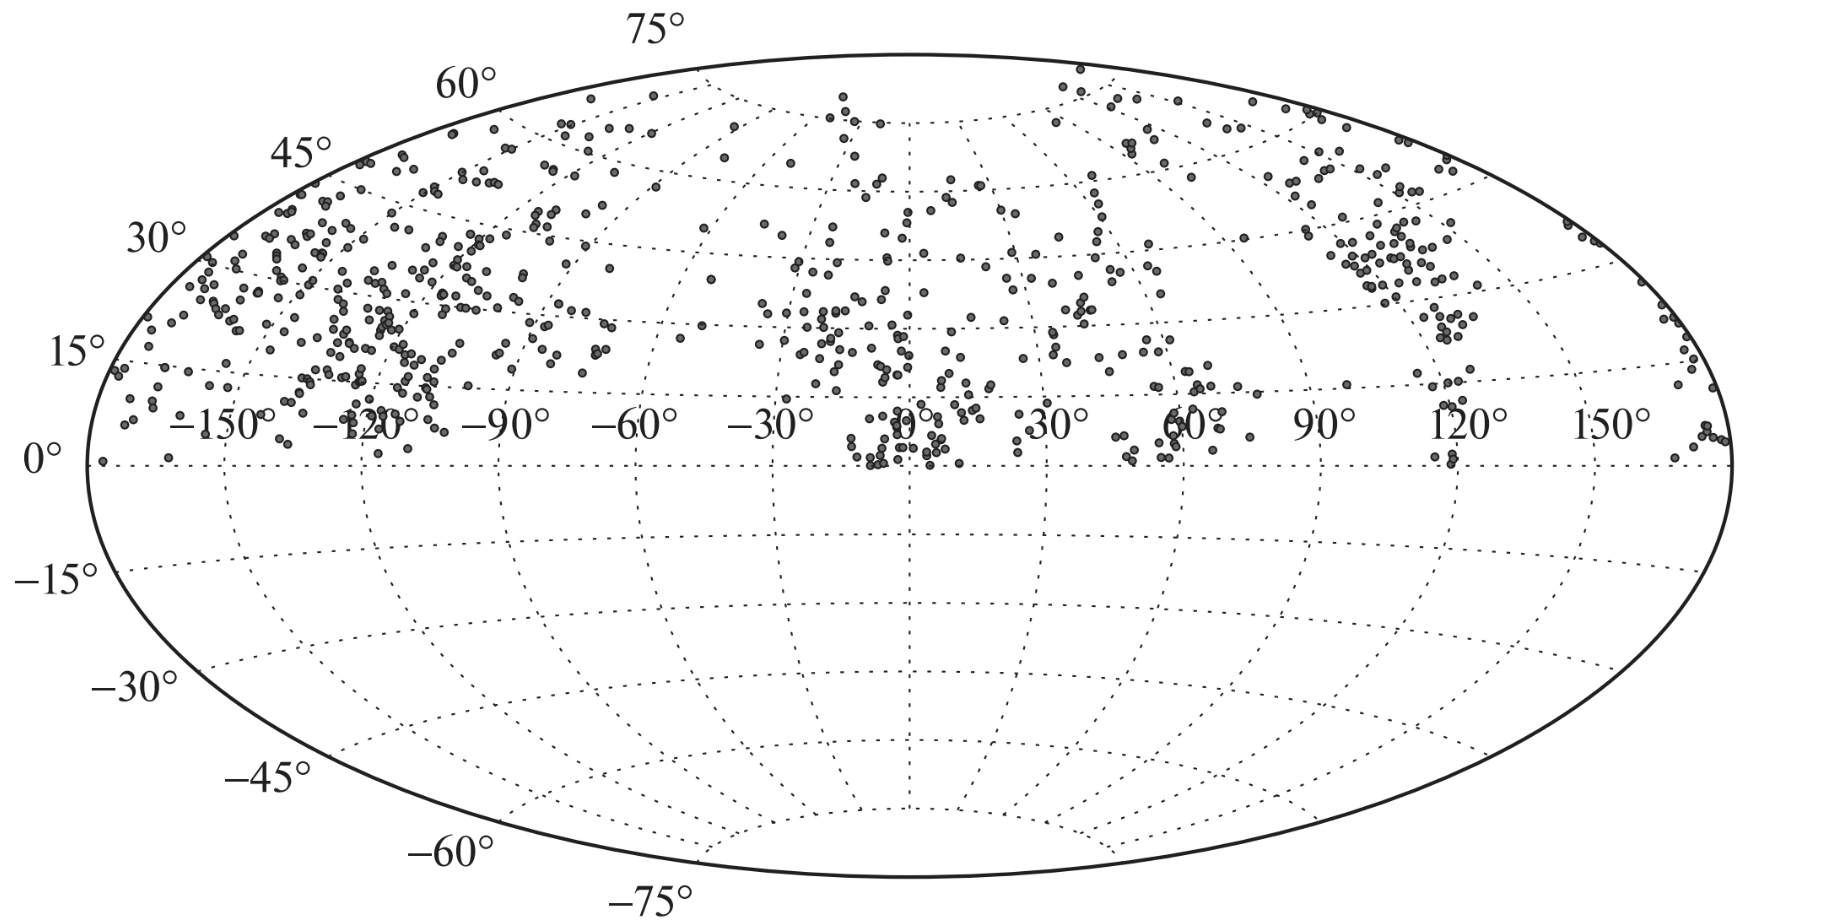
\includegraphics [scale=0.35] {khovr2018-6}
\caption{Распределение по небесной сфере (экваториальные координаты) звезд из исследования \cite{2018AstL...44..103K}. Взято из указанной работы, рис. 6.}
\label{fig:EAStars}
\end{figure}

Алгоритм выявления изображений двойных систем по shapelet-изображениям состоит из нескольких этапов.

Первый этап вычислений состоит в построении PSF для исследуемого ПЗС-кадра. В данной работе фоновые звезды для вычисления параметров PSF отбирались так, чтобы рядом с ними не было никаких других астрономических объектов. Для этого был создан специальный алгоритм, отсеивающий ситуации, когда две фоновые звезды оказывались в пределах области размером 32$\times$32 пикселя. В расчет не принимались звезды, расположенные ближе 50 пикселей от ярких звезд, чтобы избежать заметных искажений значений шейплет-коэффициентов. В итоге формировался список из 10-ти звезд, имеющих оптимальные положение и блеск: то есть они находятся ближе других звезд кадра к исследуемой звезде и не отличаются от нее по блеску более чем на $2^m$. Для каждой из этих звезд выполнялось шейплет-разложение и формировался набор коэффициентов $f_{n_1,n_2}$ по всем выбранным звездам. Для каждой точки в пространстве шейплет-коэффициентов определялось медианное значение и осуществлялась нормировка на единичный поток. В тесных звездных полях велика вероятность искажений изображений отдельных звезд фона. Поэтому использование медианных значений повышает достоверность формируемой таким способом PSF.

В результате можно попытаться аппроксимировать изображение исследуемой звезды с помощью модели двойной звезды c компонентами, имеющими координаты $x_{ph,1},y_{ph,1}$,~$x_{ph,2},y_{ph,2}$ и значения потоков $F_1$, $F_2$,  согласно соотношению~\ref{eq:binary-model}.

\begin{align}\label{eq:binary-model}
I(x,y) = I_{bgr}+F_1\cdot\sum_{n_1,n_2=0}^{\infty}f_{n_1,n_2}\cdot B_{n_1,n_2}(\beta,x,y,x_{ph,1},y_{ph,1})+ \nonumber \\
F_2\cdot\sum_{n_1,n_2=0}^{\infty}f_{n_1,n_2}\cdot B_{n_1,n_2}(\beta,x,y,x_{ph,2},y_{ph,2}).
\end{align}

Варьируя параметры $x_{ph,1},y_{ph,1}$,~$x_{ph,2},y_{ph,2}$,~$F_1$, $F_2$ методом Левенберга~--~Марквардта и зная постоянные перехода от пиксельных координат к тангенциальным, несложно получить оценки углового разделения между компонентами ($\rho$), позиционного угла ($\theta$) и разности блеска между компонентами ($\Delta m$). Эти вычисления дают оценку точности аппроксимации "--- ошибку единицы веса $\varepsilon_{w,b}$. Аналогичная процедура может быть проведена для модели, описываемой соотношением~\ref{eq:image-shapelet}. В результате вычисляется $\varepsilon_{w,s}$ "--- ошибка единицы веса для модели одиночной звезды. Естественно ожидать, что двойственность объекта даст значимое отличие $\varepsilon_{w,s}$ от $\varepsilon_{w,b}$.

На практике этот подход дает хорошие результаты либо при незначимости вариаций PSF от звезды к звезде, либо при сравнительно больших $\rho$ и малых $\Delta m$. Этот вывод был проверен на основе модельных вычислений. Если вариации параметров PSF отсутствуют (то есть относительная вариация PSF равна нулю "---  $S_{PSF}=0$), то отношение $\varepsilon_{w,s}/\varepsilon_{w,b}=2.6$ при относительном расстоянии между компонентами $\frac{\rho}{FWHM}=0.42$ и $\Delta m = 1^m$. Что дает возможность успешно детектировать двойную систему. В дальнейшем вариации параметров PSF моделировались на основе реальных ПЗС-кадров, взятых из обзора SDSS, и снимков, полученных на пулковском метровом телескопе <<Сатурн>>. Характерное значение $S_{PSF}$ для этого материала лежит в пределах от 0.1 до 0.2. Как следует из таблиц с результатами исследования \cite{2018AstL...44..103K}, при таких вариациях PSF и $\Delta m = 1^m$ отношение $\varepsilon_{w,s}/\varepsilon_{w,b}=2.0$ при $\frac{\rho}{FWHM}=0.85$. Помимо этого вычислялись оценки эллиптичности для звезд фона $e_{b}, A_{b}$ и модельной двойной звезды $e_{t}, A_{t}$. Оказалось, что  разности эллиптичности и индекса асимметрии ($\Delta e=e_{t} - e_{b}$ и $\Delta A=A_{t} - A_{b}$) начинают значимо расти уже при $\frac{\rho}{FWHM}=0.28$. Увеличение $\Delta m $ до $1.5^m$ еще больше затрудняет детектирование по отношению $\varepsilon_{w,s}/\varepsilon_{w,b}$, в то время как значения эллиптичности и индекса асимметрии  демонстрируют наличие двух компонент в изображении. Для данного моделирования принималось, что SNR=200, а ошибки определения эллиптичности и индекса асимметрии составили 0.01.

Исходя из проведенного анализа, на втором этапе вычислений детектирование двойственности проводилось на основе оценок эллиптичности и индекса асимметрии. Для звезд фона строились оценки эллиптичности и индекса асимметрии $e_{b}$, $A_{b}$ и определялись их стандартные ошибки $\varepsilon_{e_{b}}$, $\varepsilon_{A_{b}}$. Аналогичным образом вычислялись значения данных параметров для исследуемой звезды $e_{t}$, $A_{t}$ и $\varepsilon_{e_{t}}$, $\varepsilon_{A_{t}}$. Взаимные стандартные ошибки определялись как $\sigma_e^2 = \varepsilon_{e_{b}}^2+\varepsilon_{e_{t}}^2$ и $\sigma_A^2 = \varepsilon_{A_{b}}^2+\varepsilon_{A_{t}}^2$.

Далее несложно было получить разности эллиптичностей и индексов асимметрии: $e_{t} - e_{b}$ и $A_{t} - A_{b}$. Для удобства дальнейшего анализа эти разности приводились в единицах взаимных стандартных ошибок, то есть:  $S_e = (e_{t} - e_{b})/\sigma_e$ и $S_A =(A_{t} - A_{b})/\sigma_A$. В данной работе к категории потенциальных двойных систем относились звезды, для которых выполнялись неравенства: $S_e\geq3$ и/или $S_A\geq3$.

Третий этап представлял собой применение модели двойной звезды, представленной соотношением~\ref{eq:binary-model} для звезд со значимыми эллиптичностью и/или индексом асимметрии. Это дало возможность вычислить достаточно точные значения $\rho$,  ~$\theta$ и $\Delta m$ для сравнительно широких пар с относительно малыми разностями блеска.

В качестве примера в левой части рис.~\ref{fig:J0740+1706} представлено изображение звезды J0740+1706  (SDSS, фильтр u), в правой части этого рисунка можно видеть PSF, построенную с учетом шума. Для самой звезды $e_{t} =0.349\pm0.031$, а   $A_{t} = 0.597\pm0.035$. Те же величины для PSF -- $e_{b} =0.084\pm0.060$, а   $A_{b} =0.122\pm0.032$. Это приводит к значениям критических величин $S_e = 3.9$ и $S_A = 10.0$, что немедленно ведет к выводу о двойственности изображения и позволяет говорить об объекте как о потенциальной двойной системе с $\rho = 1.880''\pm0.052''$,$\theta=125.7^\circ\pm1.6^\circ$ и $\Delta m= 0.733^m\pm0.005^m$ для фильтра u.

\begin{figure}[h]
\centering
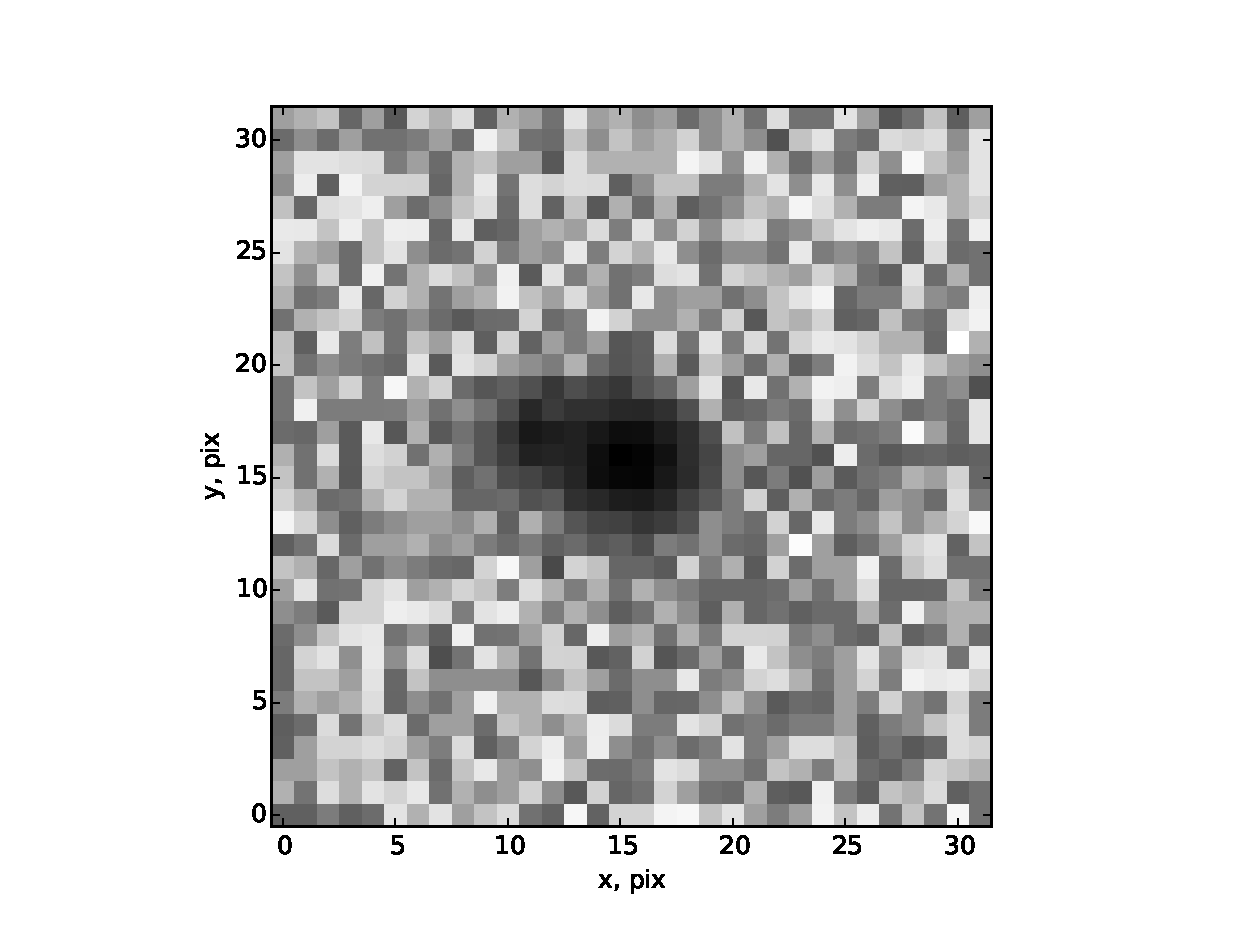
\includegraphics[width=0.48\textwidth]{J0740+1706.eps}
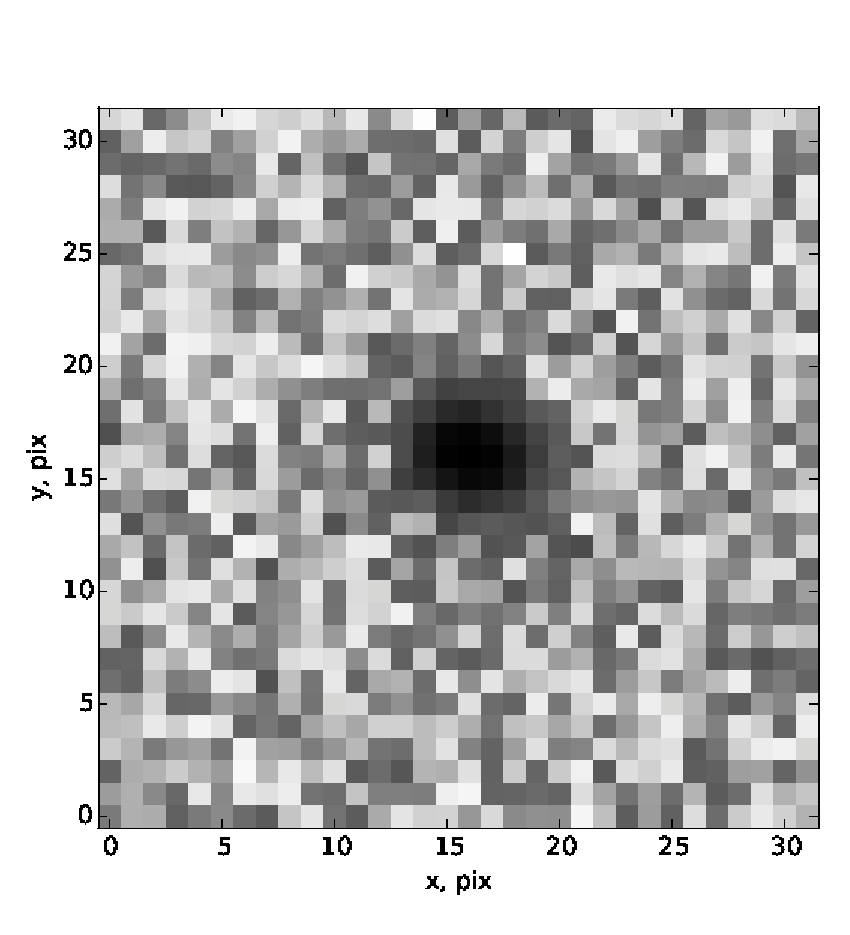
\includegraphics[width=0.48\textwidth]{J0740+1706-kernel.eps}
\caption{Слева "--- изображение звезды J0740+1706  (SDSS, фильтр u). Справа "--- PSF, построенная на основе медианных значений шейплет-коэффициентов звезд фона и оценки шума изображения. Взято из \cite{2018AstL...44..103K}, рис. 6.}
\label{fig:J0740+1706}
\end{figure}

В итоге изображения SDSS 144 из 702 исследованных звезд содержали значительные величины эллиптичности и/или асимметрии, что позволило говорить об их предположительной кратности. Отметим, что программные звезды в Gaia были отмечены флагом <<duplicate source>>, то есть относительно них стоял вопрос о кросс-идентификации. Кроме того, для девяти из этих звезд признаки двойственности удалось обнаружить и по снимкам телескопа <<Сатурн>>, эпохи наблюдений которого оказались позднее эпох кадров SDSS в среднем на 10 лет, что делает выводы о двойственности исследованных звезд более весомыми. Все результаты вычислений в форме таблиц доступны в сети. В результате для 41-ого объекта из выявленных в данном исследовании двойных систем известны значения тригонометрических параллаксов. Это позволило определить положения данных объектов на диаграмме цвет -- абсолютная звездная величина в координатах (g--i) -- $M_g$. Они показаны на рис.~\ref{fig:cmd}. В результате появилась возможность с осторожностью судить о природе звезд, двойственность которых была обнаружена.

\begin{figure}[pt]
\centering
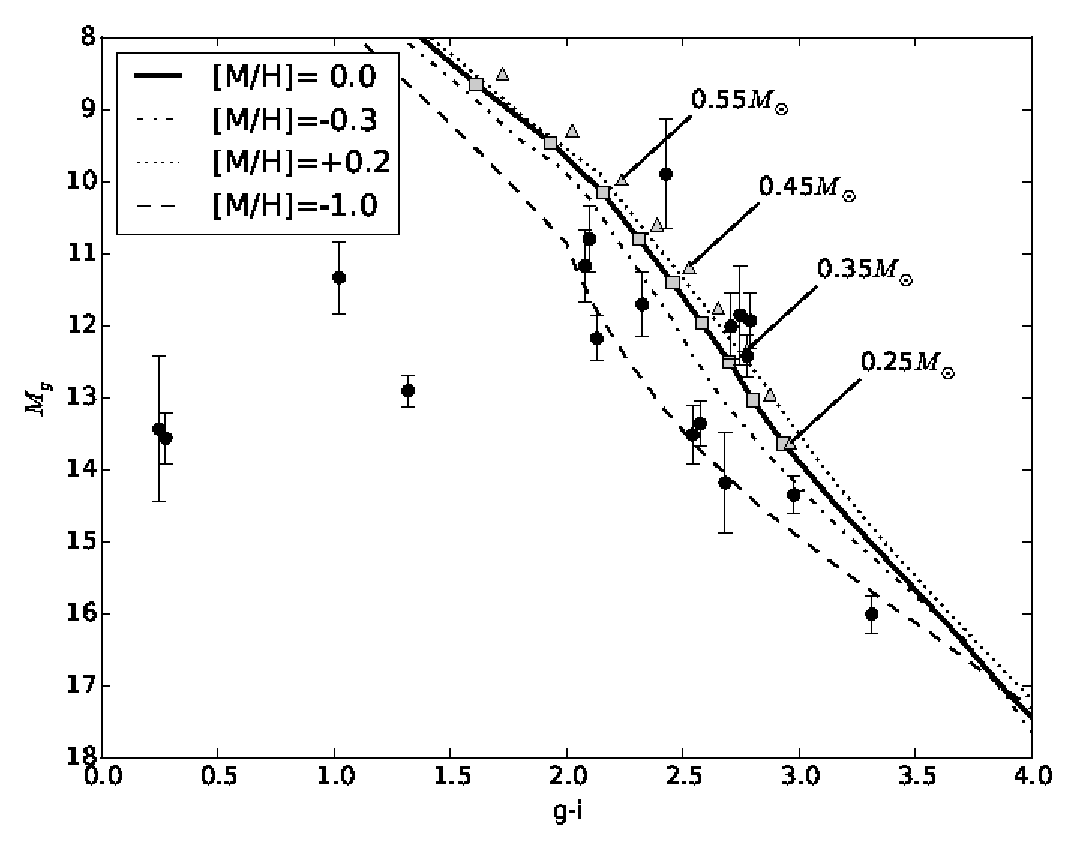
\includegraphics[width=0.7\textwidth]{cmd.eps}\\
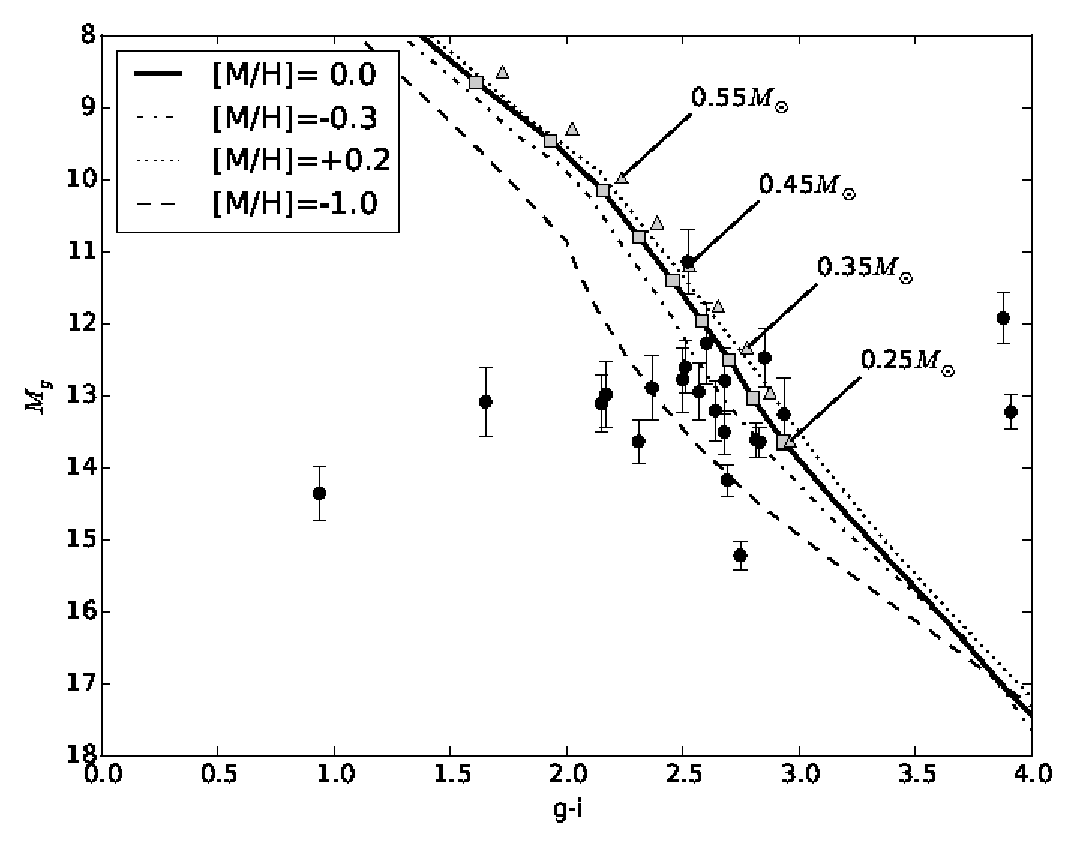
\includegraphics[width=0.7\textwidth]{cmd-asy.eps}
\caption{Положения ряда потенциальных двойных систем на диаграмме цвет -- абсолютная звездная величина (в координатах (g--i) -- $M_g$). Сверху "--- системы, детектированные по обоим признакам. Снизу "--- объекты со значимой асимметрией изображений. Взято из \cite{2018AstL...44..103K}, рис. 12.}
\label{fig:cmd}
\end{figure}

Стоит отметить, что шесть из 144 потенциальных двойных звезд оказались в каталоге WDS, однако  трех случаях двойственность была обнаружена для одной из компонент (J1137+6021W, J1451+5147E, J1540+2459W), что говорит об их вероятной тройственности. 
На изображениях ряда звезд (например, J1555-3350, рис.~\ref{fig:J1555+3350}) эллиптичность или асимметрия заметны визуально. Поэтому их двойственность представляется весьма вероятной.
\begin{figure}[h]
\centering
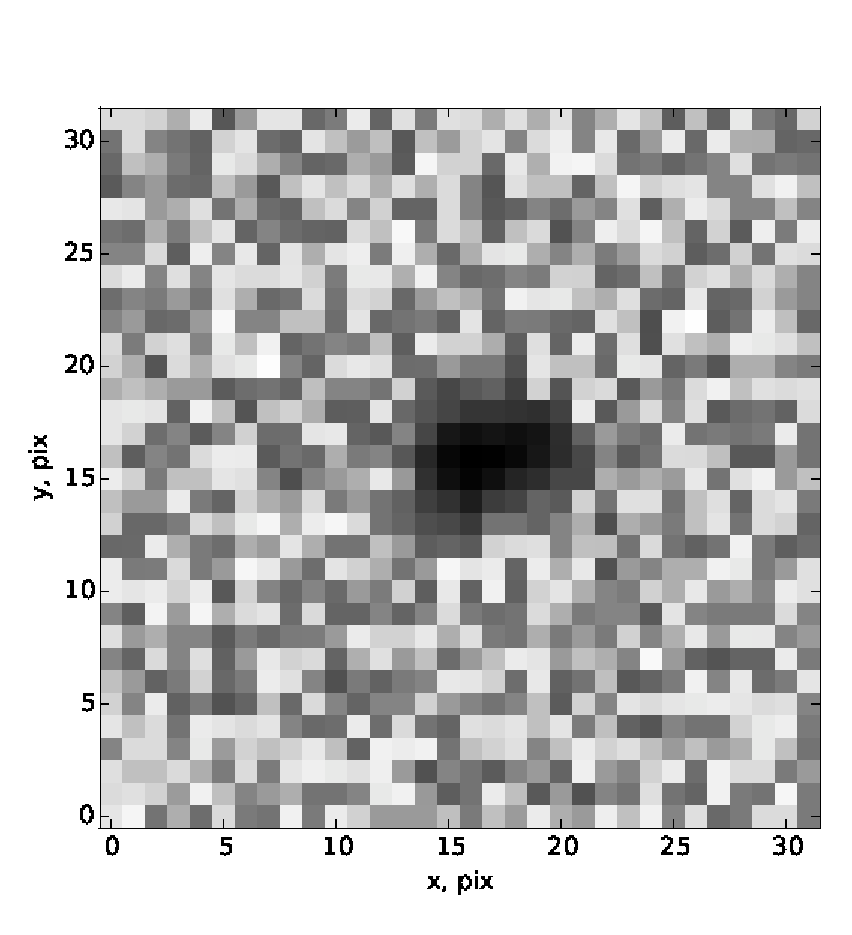
\includegraphics[width=0.48\textwidth]{J1555+3350.eps}
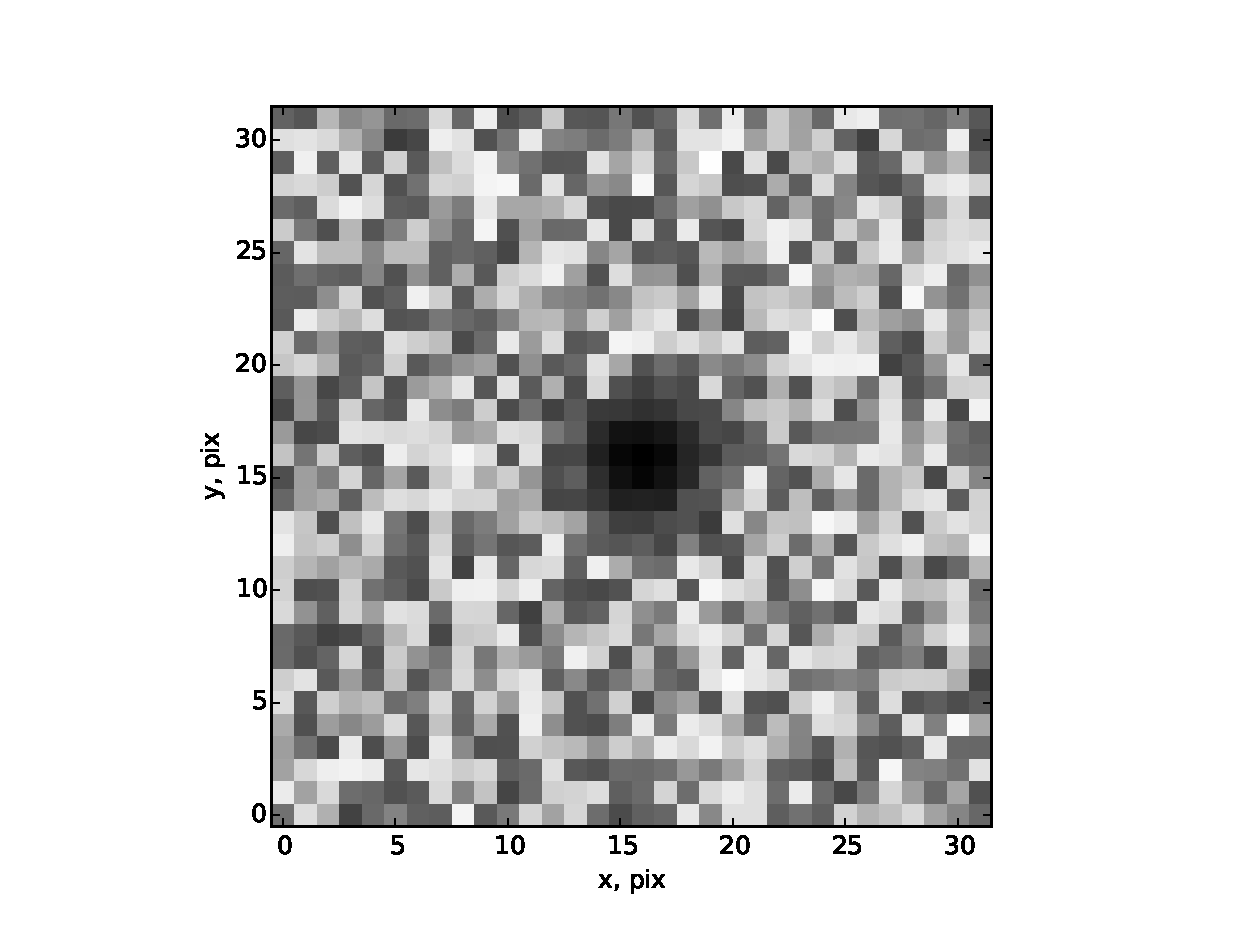
\includegraphics[width=0.48\textwidth]{J1555+3350-kernel.eps}
\caption{В левой части изображение звезды J1555+3350 (SDSS, фильтр u), в правой "--- PSF для данного кадра (с добавлением шума для наглядности). Для этого объекта $S_e=3.6$, а $S_A=7.9$. Взято из \cite{2018AstL...44..103K}, рис. 8.}
\label{fig:J1555+3350}
\end{figure}

Сведения о двойственности 138-ти звезд с большими собственными движениями, выявленных в данной работе, в других источниках не найдены. Тем не менее, говорить о том, что эти объекты точно являются двойными системами пока рано, так как не исключено случайное наложение изображения быстрой звезды на более далекий фоновый источник. Требуются дальнейшие наблюдения и анализ цифровых обзоров неба.
